% !TeX root = ../../main.tex
\section{Non-detailed reactor modelling} \label{Non-detailed}

The reactors were chosen on the basis of safety and performance. For the hydrogenation of ONT, a co-current trickle bed reactor was chosen due to the high conversion performance and absence of moving parts that might damage the expensive Pd/C catalyst. The high pressure required for the reaction can also be well controlled in a trickle bed reactor. 

Fluidised bed reactors were initially considered for the oxidation and hydrogenation of PNT derivatives, but were ruled out considering the attrition of catalyst particles due to the high flowrates. Packed-bed reactors were chosen and optimised to address its limitation of concentration and temperature gradients by controlling the residence time. Full detailed analysis for each reactor choice can be found in \cref{sec:reactorchoices}.

\begin{table}[h]
\centering
\caption{Summary of non-detailed reactors}
\label{tab:nondetailedtable}
\resizebox{\textwidth}{!}{%
\begin{tabular}{@{}llllllll@{}}
\toprule
Tag  & Type & Process & \splitcell{Volume\\ (\si{\cubic\m})} & Temperature (K) & Pressure (atm) & Duty (kW) & Conversion \\ \midrule
R201 & Co-current trickle bed & Hydrogenation & 3.93 & 333 & 5 & -137.78 & 98\% \\
R301 & Packed-bed & Oxidation & 0.02 & 750 & 1 & -77.20 & 62\% \\
R401 & Packed-bed & Oxidation & 2.75 & 750 & 1 & -56.25 & 100\% \\
R501 & Packed-bed & Hydrogenation & 0.70 & 298 & 1 & -125010 & 80\% \\
R601 & Packed-bed & Hydrogenation & 0.60 & 298 & 1 & -73.80 & 86\% \\ \bottomrule
\end{tabular}%
}
\end{table}

\subsection{R201: Hydrogenation of o-nitrotoluene}
After the production of the 3 nitrotoluene isomers, ONT is mixed with methanol and hydrogenated to o-toluidine in a co-current trickle bed reactor operating at 333K. Methanol was chosen as a solvent due to its ability to be easily separated from the product water, which can then be recycled into the reactor. Kinetic data was sourced from literature papers \cite{rajadhyaksha_solvent_1986} and operating pressure was lowered to 5 atm for safety reasons. The overall conversion for this reaction was \SI{98}{\%}.

\begin{scheme}[h]
    \centering
    \ch{ ONT + 3 H2 -> O{-}Toluidine + 2 H2O }
    \caption{ONT hydrogenation to O-TOL}
    \label{eqn: ONT hydrogenation}
\end{scheme}


The rate equation for this equation can be defined as: 
\begin{equation}
    r = k P_{H_2}^{0.3} 
    \label{ONT rate equation}
\end{equation}
 \begin{equation}
    k = 211.69 \exp \left(-\frac{45.52 \cdot 10^{3}}{RT}\right) ~(\si{\mol\per\kPa\tothe{0.3}\per\g\of{cat}\per\s})
 \end{equation}
 
\subsection{R301 \& R401: Oxidation of p-nitrotoluene}
% Andreas

\begin{wraptable}{r}{6cm}
\vspace{-\intextsep}
\centering
\caption{Corrected kinetic data for the oxidation network \cite{tan_kinetic_2010}}
\label{tab:S3-kinetics}
\begin{tabular}{@{}lS[table-format=1.3e1]S[table-format=3.2]@{}}
\toprule
Reaction & {$A$ (\si{\per\s})} & {$E_a$ (\si{\kJ\per\mol})} \\ \midrule
1        & 7.068e9  & 123.91      \\
2        & 1.503e3  & 69.54       \\
3        & 5.621e4  & 66.84       \\
4        & 3.384e6  & 81.27       \\ \bottomrule
\end{tabular}
\end{wraptable}
The oxidation of p-nitrotoluene is performed in packed-bed reactors R301 and R401, employing air as the oxidant \cite{chandalia_kinetics_1999}. The overall reaction network is shown in \cref{sch:R3} and is based on that reported for the oxidation of toluene \cite{hoorn_modelling_2005}. Kinetic information was sourced for the toluene oxidation network and corrected for the deactivation effect of the nitro- substituent using Hammett constants, resulting in rates 5.6 times slower for the nitrotoluene network \cite{partenheimer_methodology_1995}. The rate constants are shown in \cref{tab:S3-kinetics}; the corresponding rate expression for each step is first-order in the aromatic \cite{tan_kinetic_2010}, as follows:
\begin{align*}
    r_1 &= k_1 C_\text{4-nitrotoluene} & r_2 &= k_2 C_\text{4-nitrotoluene} \\
    r_3 &= k_3 C_\text{4-nitrobenzaldehyde} & r_4 &= k_4 C_\text{4-nitrobenzyl alcohol}
\end{align*}

The catalyst employed in the packed bed is cobalt phthalocyanine, with an overall loading of \SI{5}{\g\per\L} \cite{chandalia_kinetics_1999}. The feeds to the reactor are a \SI{70}{\percent\of{w/v}} 4-nitrotoluene stream, alongside air at room temperature, and it is operated at \SI{750}{\K} and \SI{1}{\atm} \cite{chandalia_kinetics_1999}. Commercial processes for the production of 4-NBA are reported with yields of \SI{88.5}{\percent} \cite{maki_benzoic_2000}; the model implemented in Aspen for the 2 oxidation reactors gave yields of \SIlist{0;0}{\percent} respectively.

\begin{scheme}[h]
    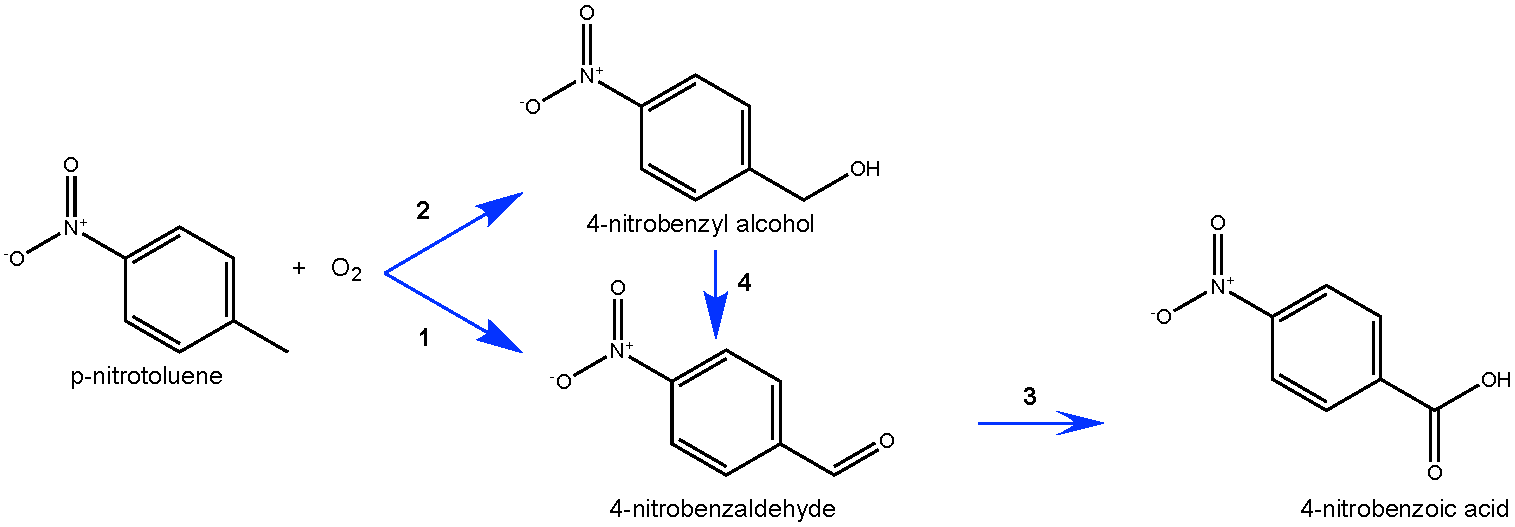
\includegraphics[width=\linewidth]{figures/R3.pdf}
    \caption{Oxidation of 4-nitrotoluene to 4-nitrobenzaldehyde, and subsequently to 4-nitrobenzoic acid}
    \label{sch:R3}
\end{scheme}

\subsection{R501 \& R601: Hydrogenation of nitrobenzaldehyde and nitrobenzoic acid}

\begin{scheme}[h]
    \centering
    \ch{ NBA + HCOOH -> ABA + CO2 + H2O }
    \\
    \ch{ NBAH + HCOOH -> ABAH + CO2 + H2O }
    \caption{Hydrogenation of NBA and NBAH to ABA and ABAH}
    \label{eqn: ONT hydrogenation}
\end{scheme}

The hydrogenation of p-nitrobenzaldehyde and p-nitrobenzoic acid were carried out in methanol solvent with formic acid as the reducing agent. The reaction was carried out at room temperature and 1 atm. 5\% w/w Pt/C was chosen as the desired catalyst to speed up the reaction due to its reusability benefits while maintaining its catalytic performance \cite{rahman_fast_2020}. The overall yield for 4-ABA and 4-ABH were 86\% and 80\% respectively as reported by \textcite{gowda_catalytic_2000}.

